\subsection{Enhanced Image vs original image}

\subsection{Gaussian Filter on Edge Image}
If images are skewed or angled, this step does not work so well. Also, for small images and other images which has low blur around plate regions enhanced margin is low. Figure \ref{fig:EnhanceResult1}, \ref{fig:EnhanceResult2}, \ref{fig:EnhanceResult3} and \ref{fig:EnhanceResult4} demonstrate result of this step.

\begin{figure}
\begin{subfigure}{0.5\textwidth}
    \centering
    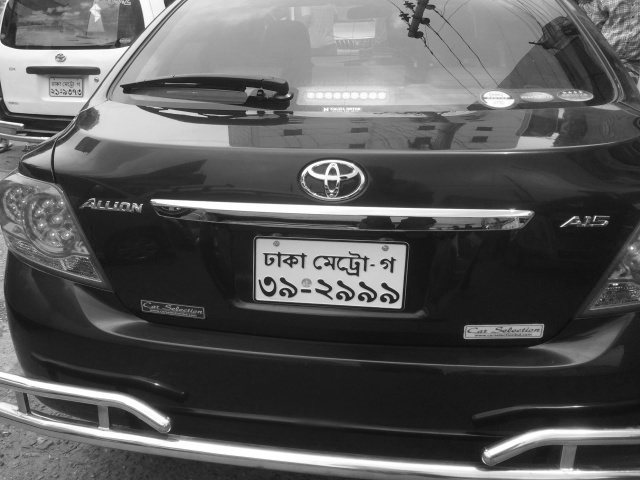
\includegraphics[width=0.9\linewidth]{./img/experiment/stage.2/angle3}
    \caption{Original image}
\end{subfigure}
\begin{subfigure}{0.5\textwidth}
    \centering
    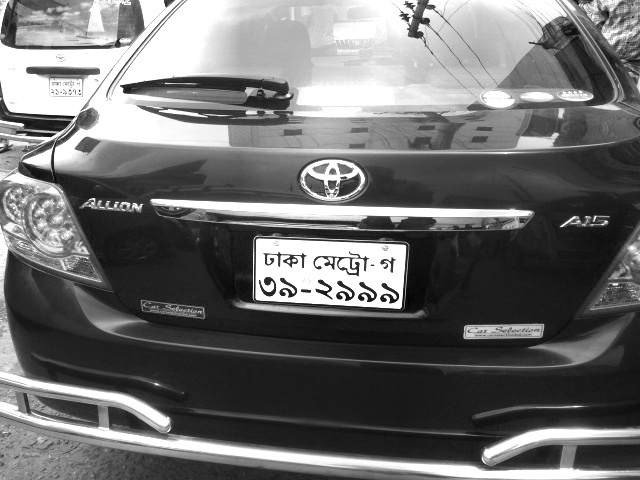
\includegraphics[width=0.9\linewidth]{./img/experiment/stage.5/angle3}
    \caption{Blurry image}
\end{subfigure}
\caption{Gaussian filter on good plate}
\label{fig:EnhanceResult1}
\end{figure}

\begin{figure}
\begin{subfigure}{0.5\textwidth}
    \centering
    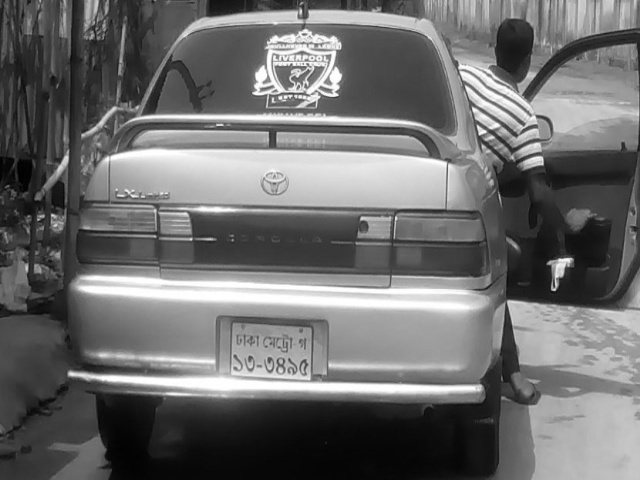
\includegraphics[width=0.9\linewidth]{./img/experiment/stage.2/light}
    \caption{Original image}
\end{subfigure}
\begin{subfigure}{0.5\textwidth}
    \centering
    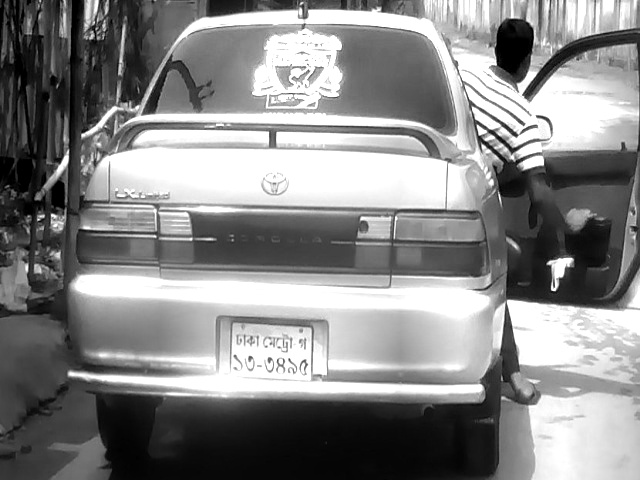
\includegraphics[width=0.9\linewidth]{./img/experiment/stage.5/light}
    \caption{Blurry image}
\end{subfigure}
\caption{Gaussian filter on plate with reflection}
\label{fig:EnhanceResult2}
\end{figure}

\begin{figure}
\begin{subfigure}{0.5\textwidth}
    \centering
    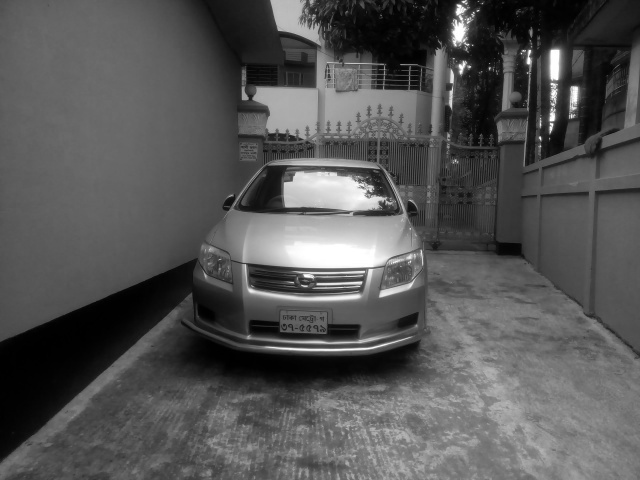
\includegraphics[width=0.9\linewidth]{./img/experiment/stage.2/small}
    \caption{Original image}
\end{subfigure}
\begin{subfigure}{0.5\textwidth}
    \centering
    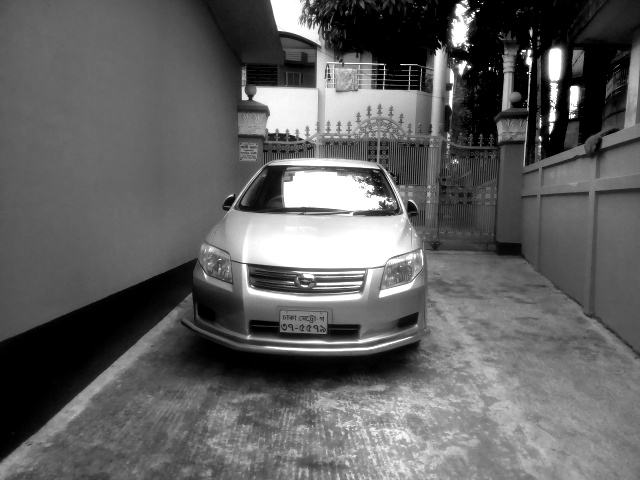
\includegraphics[width=0.9\linewidth]{./img/experiment/stage.5/small}
    \caption{Blurry image}
\end{subfigure}
\caption{Gaussian filter on small plate}
\label{fig:EnhanceResult3}
\end{figure}


\begin{figure}
\begin{subfigure}{0.5\textwidth}
    \centering
    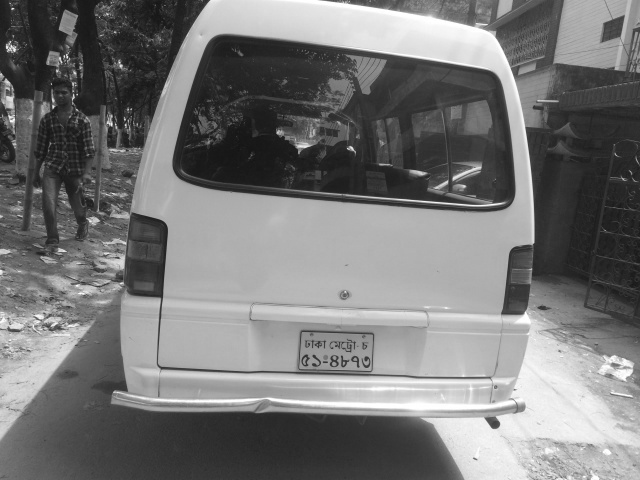
\includegraphics[width=0.9\linewidth]{./img/experiment/stage.2/angle}
    \caption{Original image}
\end{subfigure}
\begin{subfigure}{0.5\textwidth}
    \centering
    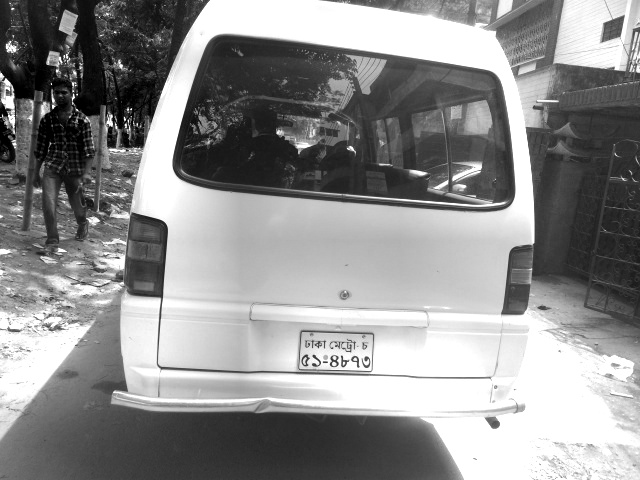
\includegraphics[width=0.9\linewidth]{./img/experiment/stage.5/angle}
    \caption{Blurry image}
\end{subfigure}
\caption{Gaussian filter on plate that is angled slightly}
\label{fig:EnhanceResult4}
\end{figure}
